\documentclass{article}

\usepackage[%
    left=0.5in,%
    right=0.5in,%
    top=0.5in,%
    bottom=0.5in,%
]{geometry}%
\usepackage{minitoc}
\usepackage{multicol}
\usepackage{graphicx}
\usepackage{fixltx2e}
\usepackage{listings}
\usepackage{color}
\usepackage{hyperref}
    \hypersetup{ colorlinks = true, linkcolor = blue }
\usepackage{blindtext}
\definecolor{lightgray}{gray}{0.9}
\graphicspath{ {./} }

\newcommand{\inlinecode}[2]{\colorbox{lightgray}{\lstinline
[language=#1]$#2$}}
\newcommand{\worddef}[1]{\hyperref[sec:reference]{\textit{#1}}}

\usepackage{blindtext}
\title{G53DEV Final report}
\author{Augustinas Jokubauskas (psyaj1)}

\begin{document}

\maketitle

\begin{flushleft}
When looking at github commits, some might say username of Knightls or Augustinas, that happened because I had configured github incorrectly. All the charts are taken from and can be confirmed on \href{https://npm-stat.com}{npm-stat}
\end{flushleft}

\pagebreak

\tableofcontents

\newpage

\section{Dlister}

\subsection{About}

\begin{flushleft}
This project was created on \textbf{05/02/2017} and can be found on \href{https://github.com/WhoAteDaCake/dlister}{Github}. \\
It's a cli tool, which allows to quickly and easily list directory trees and files within them. It's build on top of node.js which allows it to be used as a universal tool with extremely simple installation on a large number of operating systems. Dlister also has a stackoverflow integration allowing for painless project layout display when creating a question. I am currently the sole maintainer of the project, which lead to development being slowed down recently, however there are plans for a complete rewrite in ocaml using bucklescript compiler to transform it to javascript. This would mean being able to utilise ocaml's type system to produce better quality code.
\end{flushleft}

\subsection{Example usage}

\begin{multicols}{2}
  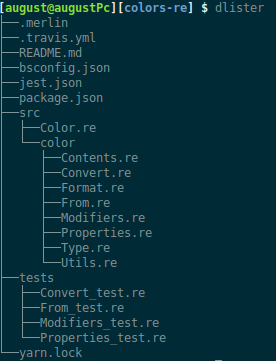
\includegraphics[scale=0.5]{dlister_use.png}
  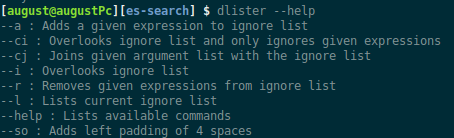
\includegraphics[scale=0.8]{dlister_help.png}
\end{multicols}

\subsection{Statistics}
\begin{flushleft}
Between 05/02/2017 and 26/09/2018 package has been downloaded \textbf{2297} times
\end{flushleft}

\begin{center}
  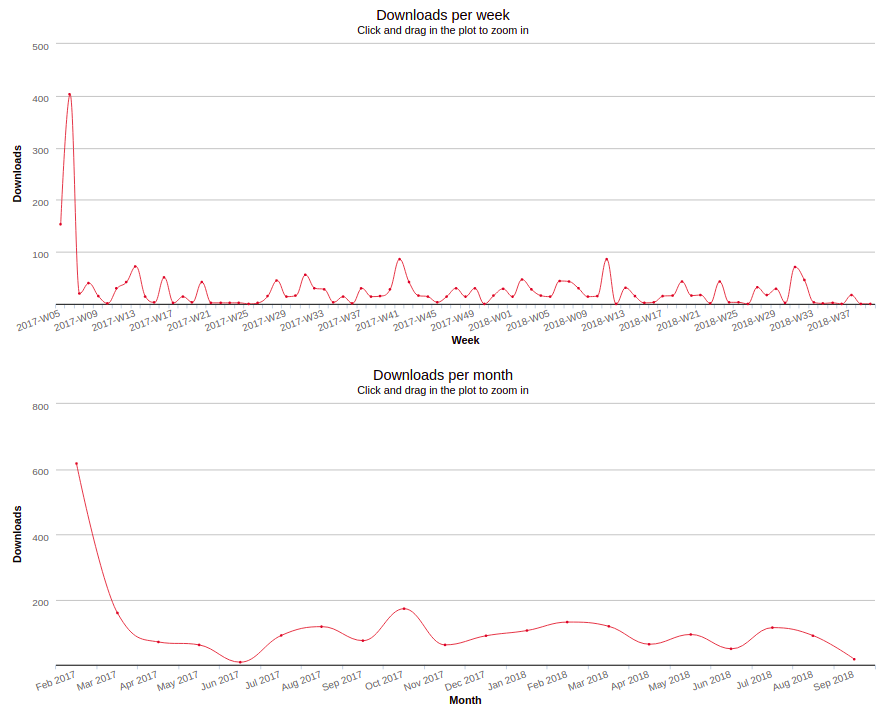
\includegraphics[scale=0.4]{dlister.png}
\end{center}

\pagebreak




\end{document}
